\begin{refsection}

\chapter{Fission tracks}\label{ch:fissiontracks}

\texttt{IsoplotR} accepts three types of fission track data:

\begin{enumerate}
\item{`EDM':} \textzeta, err[\textzeta],
  \textrho\textsubscript{D}, err[\textrho\textsubscript{D}], 
  N\textsubscript{s}, N\textsubscript{i}
\item{`ICP (\textzeta)':} \textzeta, err[\textzeta], spot size
  (\textmu{m}), U\textsubscript{1}, err[U\textsubscript{1}],
  U\textsubscript{2}, err[U\textsubscript{2}], $\ldots$,
  U\textsubscript{n}, err[U\textsubscript{n}]
\item{`ICP (absolute)':} mineral, spot size (\textmu{m}),
  U\textsubscript{1}, err[U\textsubscript{1}], U\textsubscript{2},
  err[U\textsubscript{2}], $\ldots$, U\textsubscript{n},
  err[U\textsubscript{n}]
\end{enumerate}

\noindent \textzeta, err[\textzeta], \textrho\textsubscript{D},
err[\textrho\textsubscript{D}], and `spot size' are scalars, whereas
N\textsubscript{s}, N\textsubscript{i}, U\textsubscript{i} and
err[U\textsubscript{i}] are vectors. `mineral' is a text string that
either equals \texttt{apatite} or \texttt{zircon}.  The three formats
represent two different approaches to fission track dating:

\begin{enumerate}
\item The External Detector Method (EDM) implements the neutron
  irradiation method that was previously introduced in
  Section~\ref{sec:fission-tracks}.
\item The `ICP' method uses LA-ICP-MS (see
  Section~\ref{sec:mass-specs}) to determine the
  \textsuperscript{238}U-content of fission track samples.  The main
  reasons for this change are the increased throughput achieved by not
  having to irradiate samples and the ease of double-dating apatite
  and zircon with the U-Pb method.
\end{enumerate}

\section{The external detector method}
\label{sec:EDM}

Recall the fission track age equation from
Section~\ref{sec:fission-tracks}:
\begin{equation}
t =
\frac{1}{\lambda_{38}}\ln\left(1+\frac{g_i}{g_s}
\lambda_{38}\zeta\rho_d\frac{N_s}{N_i}\right)
\label{eq:tzeta2}
\end{equation}

The fission track method has been a test bed of statistical approaches
that have subsequently been adopted by other chronometers. A case in
point is the radial plot, which is uniquely suited to deal with the
large and highly variable (`heteroscedastic') counting uncertainties
of fission track data. Spontaneous fission is accurately described by
a Poisson distribution. For young and/or uranium-poor samples, there
is a finite probability that the spontaneous track count is zero for
some grains.  To accommodate such zero values, it is customary to use
an arcsine transformation for radial plots instead of the usual
logarithmic transformation \citep{galbraith1990a}:
\begin{equation}
z_j = \arcsin\sqrt{\frac{N_{sj} + 3/8}{N_{sj}+N_{ij}+3/4}}
\label{eq:zj}
\end{equation}

\noindent and
\begin{equation}
\sigma_j = \frac{1}{2\sqrt{N_{sj}+N_{ij}+1/2}}
\label{eq:sj}
\end{equation}

The arithmetic mean is not a reliable estimator of the true age, for a
similar reason why the arithmetic mean is not the best estimator of
the average U--Th--He composition and age. The Poisson distribution is
negatively skewed, and this biases the arithmetic mean. The solution
is similar as for the U--Th--He method, namely:

\begin{enumerate}
\item Take the average logarithm of the spontaneous and induced
  track densities.
\item Compute the fission track age the corresponds to this average
  ratio.
\end{enumerate}

This procedure again gives rise to a `central age'. Fission track data
are often overdispersed with respect to the Poisson counting
uncertainties, and this dispersion carries important thermal history
information. It is therefore customary to compute the average track
density ratio using a model-3 style random effects model, in which the
true $\rho_s/\rho_i$-ratio is assumed to follow a log-normal
distribution with location parameter $\mu$ and scale parameter
$\sigma$ \citep{galbraith1993}:
\begin{equation}
\ln\left[\frac{\rho_s}{\rho_i}\right] \sim \mathcal{N}(\mu,\sigma^2)
\label{eq:logrhosrhoi}
\end{equation}

This model gives rise to a two-parameter log-likelihood function:
\begin{equation}
  \mathcal{L}(\mu,\sigma^2) = \sum\limits_{j=1}^{n}
  \ln f_j(\mu,\sigma^2)
\label{eq:Lcentral}
\end{equation}

\noindent where the probability mass function $f_j(\mu,\sigma^2)$ is
defined as:
\begin{equation}
  f_j(\mu,\sigma^2) = {{N_{sj}+N_{ij}}\choose{N_{sj}}}
  \int\limits_{-\infty}^{\infty} \frac{e^{\beta N_{sj}} \left( 1 +
    e^\beta \right)^{-N_{sj}-N_{ij}}} {\sigma\sqrt{2\pi}
    e^{(\beta-\mu)^2/(2\sigma^2)}} d\beta
  \label{eq:fjms}
\end{equation}

\noindent in which the fission track count ratios are subject to two
sources of variation: the Poisson counting uncertainty and an
`(over)dispersion' factor $\sigma$.  Maximising Eq. \ref{eq:Lcentral}
results in two estimates $\hat{\mu}$ and $\hat{\sigma}$ and their
respective standard errors.  Substituting $\exp[\hat{\mu}]$ for
$N_s/N_i$ in Equation~\ref{eq:tzeta2} produces the desired central
age. $\hat{\sigma}$ estimates the overdispersion, and quantifies the
excess scatter of the single grain ages which cannot be explained by
the Poisson counting statistics alone. This dispersion can be just as
informative as the central age itself, as it encodes geologically
meaningful information about the compositional heterogeneity and
cooling history of the sample.

\section{LA-ICP-MS based fission track dating}
\label{sec:ICPFT}

The EDM continues to be the most widely used analytical protocol in
fission track dating. However, over the past decade, an increasing
number of laboratories have abandoned it and switched to LA-ICP-MS as
a means of determining the uranium concentration of datable minerals,
thus reducing sample turnover time and removing the need to handle
radioactive materials\citep{hasebe2004, chew2012, vermeesch2017}. The
statistical analysis of ICP-MS based FT data is less straightforward
and less well developed than that of the EDM. The latter is based on
simple ratios of Poisson variables, and forms the basis of a large
edifice of statistical methods which cannot be directly applied to
ICP-MS based data. The following paragraphs summarise
\citet{vermeesch2017}'s solution to these issues, as implemented in
\texttt{IsoplotR}.\\

Two analytical approached are being used in ICP-based fission track
geochronology, which each correspond to a different data format:

\begin{enumerate}
\item The `absolute dating' method is based on
  Equation~\ref{eq:tFT}:
  \begin{equation}
    {t} = \frac{1}{\lambda_D}
    \ln \left(1 + \frac{\lambda_D}{\lambda_f}\frac{N_s}{[{U}] A_s R_e ~ q}\right)
    \label{eq:tICP}
  \end{equation}

  where $N_s$ is the number of spontaneous tracks counted over an area
  $A_s$, $q$ is an `efficiency factor' \citep[$\sim$0.93 for apatite and
    $\sim$1 for
    zircon,][]{iwano1998,enkelmann2003,jonckheere2003b,soares2013} and
  $[{U}]$ is the $^{238}$U-concentration (in atoms per unit volume)
  measured by LA-ICP-MS. Equation \ref{eq:tICP} requires an explicit
  value for $\lambda_f$ and assumes that the etchable range ($R_e$) is
  accurately known \citep{soares2014}.

\item The \textzeta-calibration method folds the etch efficience,
  decay constant and etchable range into a $\zeta$-calibration factor
  akin to that used in the EDM:
  \begin{equation}
    {t} = \frac{1}{\lambda_D}
    \ln \left(1+\frac{1}{2}\lambda_D{\zeta}_{ICP}\frac{N_s}{A_s[{U}]}\right)
    \label{eq:tzetahatICP}
  \end{equation}

  in which ${\zeta}_{ICP}$ is determined by analysing a standard of
  known FT age \citep{hasebe2004}. Note that, in contrast with the
  `absolute' dating method, the $\zeta$-calibration method allows
  $[{U}]$ to be expressed in any concentration units (e.g., ppm or
  wt\% of total U) or could even be replaced with the measured U/Ca-,
  U/Si- or U/Zr-ratios produced by the ICP-MS instrument.
\end{enumerate}

\section{Compositional zoning}\label{sec:zoning}

Uranium-bearing minerals such as apatite and zircon often exhibit
compositional zoning, which must either be removed or quantified in
order to ensure unbiased ages. Two approaches are being used to deal
with this issue:

\begin{enumerate}
\item The effect of compositional zoning can be \emph{removed} by
  covering the entire counting area with one large laser spot
  \citep{soares2014} or a raster \citep{hasebe2004}. The uncertainty
  of $[{U}]$ is then simply given by the analytical uncertainty of the
  LA-ICP-MS instrument, which typically is an order of magnitude lower
  than the standard errors of induced track counts in the EDM.
\item Alternatively, the uranium-heterogeneity can be
  \emph{quantified} by analysing multiple spots per analysed grain
  \citep{hasebe2009}. This is why \texttt{IsoplotR} accommodates
  multiple uranium measurements per aliquot (U\textsubscript{1},
  err[U\textsubscript{1}], $\ldots$, U\textsubscript{n},
  err[U\textsubscript{n}])\\

  It is commonly found that the variance of the different
  uranium-measurements within each grain far exceeds the formal
  analytical uncertainty of each spot measurement. \texttt{IsoplotR}
  assumes that this dispersion is constant across all aliquots and
  follows a log-normal distribution:
  \begin{equation}
    \ln[U_{jk}] \sim \mathcal{N}(\mu_j,\sigma^2+s[U]_{jk}^2)
    \label{eq:lognorm}
  \end{equation}

  where ${U}_{jk}$ is the $k$\textsuperscript{th} (out of $n_j$)
  uranium concentration measurement, $s[U]_{jk}$ is its standard
  error, and and $\mu_j$ and $\sigma^2$ are the (unknown) mean and
  variance of a Normal distribution. Note that $\mu_j$ is allowed to
  vary from grain to grain but $\sigma$ is not.  $\mu_j$ and $\sigma$
  can be estimated using the method of maximum likelihood, and the
  corresponding geometric mean uranium concentrations ($\exp[\mu_j]$)
  directly plugged into Equation~\ref{eq:tICP}.
\end{enumerate}

To plot ICP-MS based fission track data on a radial plot, we can
replace Eqs.~\ref{eq:zj} and \ref{eq:sj} with
\begin{align}
  z_j & = \ln ({t}_j) \mbox{,}   \label{eq:zj2} \\
  \mbox{and~} s_j & = \sqrt{ 
    \left(\frac{s[{\zeta}]}{{\zeta}}\right)^2 +
    \left(\frac{s[{U}]}{{U}}\right)^2 +
    \frac{1}{N_s}
  }   \label{eq:sj2}
\end{align}

respectively \citep{galbraith2010b}. Alternatively, a square root
transformation may be more appropriate for young and/or U-poor
samples:
\begin{align}
  z_j & = \sqrt{{t}_j} \mbox{,}   \label{eq:zj3} \\
  \mbox{and~} s_j & = s[{t}_j]\bigg/\left(2\sqrt{{t}_j}\right)
  \label{eq:sj3}
\end{align}

\noindent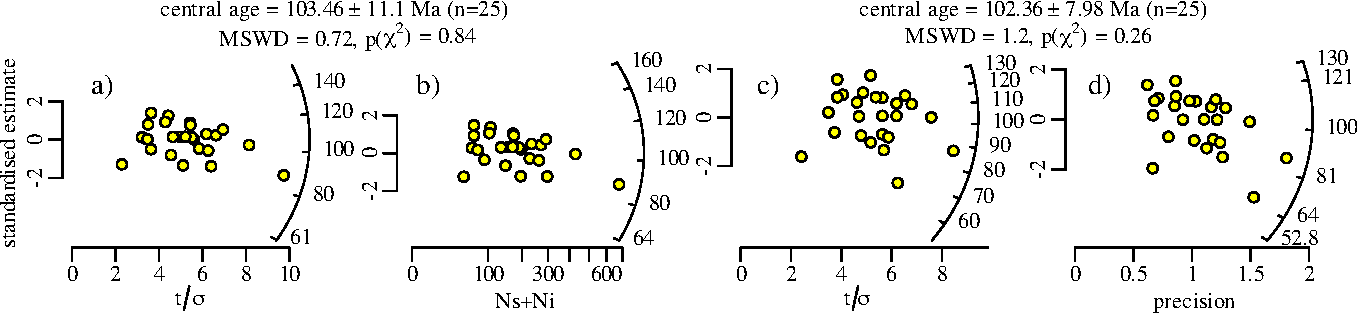
\includegraphics[width=\linewidth]{../figures/FTradial.pdf}
\begingroup \captionof{figure}{Radial plots of EDM-based fission track
  data using the a) logarithmic and b) arcsine transformation; and of
  ICP-based fission track data using the c) logarithmic and d) square
  root transformation.}  \endgroup

\section{Zero track counts}
\label{sec:zeroICP}

The standard error of a single grain fission track age estimate can be
derived by standard error propagation.  For the EDM, this yields:
\begin{equation}
s[{t}] \approx {t} \sqrt{ 
  \left(\frac{s[{\zeta}]}{{\zeta}}\right)^2 +
  \left(\frac{s[{\rho_D}]}{{\rho_D}}\right)^2 +
  \frac{1}{N_s} + \frac{1}{Ni}
}
\label{eq:stEDM}
\end{equation}

\noindent which returns an infinite uncertainty if either $N_s$ or
$N_i$ is zero. For the EDM, this problem is adequately addressed by
adding half a count to both the spontaneous and induced track count:
\begin{equation}
s[{t}] \approx {t} \sqrt{ 
  \left(\frac{s[{\zeta}]}{{\zeta}}\right)^2 +
  \left(\frac{s[{\rho_D}]}{{\rho_D}}\right)^2 +
  \frac{1}{N_s+\frac{1}{2}} + \frac{1}{N_i+\frac{1}{2}}
}
\label{eq:stEDM0}
\end{equation}

This correction avoids the problem with zero or small counts whilt
only having a minor effect on the accuracy of the
estimate. Unfortunately this simple trick does not work for ICP-based
fission track data, whose uncertainty estimates are given by (for the
absolute dating approach):
\begin{equation}
s[{t}] \approx {t} \sqrt{ 
  \left(\frac{s[{U}]}{{U}}\right)^2 +
  \frac{1}{N_s}
}
\label{eq:shatt4}
\end{equation}

Adding half a count to the spontaneous fission track count would
introduce more or less bias depending on whether the grain is poor or
rich in uranium. One pragmatic solution to this problem is to
approximate the ICP-MS based uranium concentration measurement with an
`equivalent induced track density', using the following linear
transformation:
\begin{equation}
\hat{N}_{ij} = \rho_j A_{sj} [{U}_j]
\end{equation}

\noindent where $A_{sj}$ is the area over which the spontaneous tracks
of the j$^{th}$ grain have been counted and $\rho_j$ plays a similar
role as $\rho_d$ in Eq.~\ref{eq:tzeta}. From the requirement that the
variance of a Poisson-distributed variable equals its mean, it follows
that:
\begin{equation}
\hat{N}_{ij} = \rho_j^2 A_{sj}^2 s[{U}_j]^2
\end{equation}

\noindent from which it is easy to determine $\rho_j$. Thus the ICP-MS
data have effectively been converted in to EDM data, and can be
subjected to the same treatment as EDM data.

\printbibliography[heading=subbibliography]

\end{refsection}
